\graphicspath{{./ch_LDE/figures/}}

\chapter[Heralded entanglement and unconditional teleportation between solid-state qubits separated by three metres]{Heralded entanglement and unconditional teleportation between solid-state qubits separated by three metres}
\label{ch:LDE}

\begin{center} 
    \vspace{-1cm} {H.~Bernien, W.~Pfaff, B.~Hensen,  M.S.~Blok, T.H.~Taminiau, S.B.~van Dam, G.~Koolstra, L.~Robledo, M.J. ~Tiggelman, R.N. ~Schouten, M.~Markham, D.J.~Twitchen, L.~Childress, and R.~Hanson} 
\end{center}

{\renewcommand{\thefootnote}{}\footnote{The results in this chapter have been published in
    {\em Nature} \textbf{497}, 86 (2013) and {\em Science} \textbf{345}, 532 (2014).}}

\vspace{-0.5cm} 
Quantum entanglement between spatially separated objects is a unique resource for quantum information processing and communication. Entangled qubits can be used to establish private information or implement quantum logical gates~\cite{Nielsen__2000,Raussendorf_Phys.Rev.Lett._2001}. Such capabilities are particularly useful when the entangled qubits are spatially separated~\cite{Moehring_Nature_2007,Ritter_Nature_2012,Hofmann_Science_2012}, opening the opportunity to create highly connected quantum networks~\cite{Kimble_Nature_2008} or extend quantum cryptography to long distances~\cite{Duan_Nature_2001,Childress_Phys.Rev.Lett._2006}. Here we present two key experiments towards the realisation of long-distance quantum networks with solid-state quantum registers. Firstly, we have entangled two electron spin qubits in diamond that are separated by a three-metre distance. Our robust entangling protocol is based on local creation of spin-photon entanglement and a subsequent joint measurement of the photons to herald spin-spin entanglement. The resulting shared Bell-pair between the two nodes then enables the unconditional teleportation of a single nuclear spin state by combining a deterministic Bell-state measurement with real-time feed-forward. These results establish diamond spin qubits as a prime candidate for the realization of quantum networks for quantum communication and network-based quantum computing

% Detection of the photons heralds the projection of the spin qubits onto an entangled state. We verify the resulting non-local quantum correlations by performing single-shot readout~\cite{Robledo2011} on the qubits in different bases. The long-distance entanglement reported here can be combined with recently achieved initialisation, readout and entanglement operations~\cite{Robledo2011,Neumann2010a,Neumann2008,Maurer2012,Pfaff2012} on local long-lived nuclear spin registers, enabling deterministic long-distance teleportation, quantum repeaters and extended quantum networks.

\clearpage

\section{Introduction}

A quantum network can be constructed by using entanglement to connect local processing nodes, each containing a register of well-controlled and long-lived qubits~\cite{Kimble_Nature_2008}. Solids are an attractive platform for such registers, as the use of nano-fabrication and material design may enable well-controlled and scalable qubit systems~\cite{Ladd_Nature_2010}. The potential impact of quantum networks on science and technology has recently spurred research efforts towards generating entangled states of distant solid-state qubits~\cite{Togan_Nature_2010,Gao_Nature_2012,DeGreve_Nature_2012,Bernien_Phys.Rev.Lett._2012,Sipahigil_Phys.Rev.Lett._2012,Patel_NatPhoton_2010,Flagg_Phys.Rev.Lett._2010}.

A prime candidate for a solid-state quantum register is the nitrogen-vacancy (NV) defect centre in diamond. The NV centre combines a long-lived electronic spin (S=1) with a robust optical interface, enabling measurement and high-fidelity control of the spin qubit~\cite{Togan_Nature_2010,Fuchs_Science_2009,Lange_Science_2010,vanderSar_Nature_2012}. Furthermore, the NV electron spin can be used to access and manipulate nearby nuclear spins~\cite{Robledo_Nature_2011,Neumann_Science_2010,Neumann_Science_2008,Maurer_Science_2012,Pfaff_NatPhys_2013}, thereby forming a multi-qubit register. To use such registers in a quantum network requires a mechanism to coherently connect remote NV centres.

!! make more general to include teleportation!! Here we demonstrate the generation of entanglement between NV centre spin qubits in distant setups. We achieve this by combining recently established spin initialisation and single-shot readout techniques~\cite{Robledo_Nature_2011} with efficient resonant optical detection and feedback-based control over the optical transitions, all in a single experiment and executed with high fidelity. These results put solid-state qubits on par with trapped atomic qubits~\cite{Moehring_Nature_2007,Ritter_Nature_2012,Hofmann_Science_2012} as highly promising candidates for implementing quantum networks.

Our experiment makes use of two NV spin qubits located in independent low-temperature setups separated by 3 metres (Fig.\,\ref{fig:LDE-fig1-setup}). We encode the qubit basis states $\ket{\up}$ and $\ket{\down}$ in the NV spin sub-levels $\mszero$ and $\msmone$, respectively. Each qubit can be independently read out by detecting spin-dependent fluorescence in the NV phonon side band (non-resonant detection)~\cite{Robledo_Nature_2011}. The qubits are individually controlled with microwave pulses applied to on-chip strip-lines~\cite{Lange_Science_2010}. Quantum states encoded in the qubits are extremely long-lived: using dynamical decoupling techniques~\cite{Lange_Science_2010} we obtain a coherence time exceeding 10$\,$ms (Fig.\,\ref{fig:LDE-fig1-DD}).

\begin{figure}[tp]
	\centering
	\includegraphics{fig1_entanglement_setup}
	\caption{\label{fig:LDE-fig1-setup} \textbf{Experimental setup.} a Each nitrogen vacancy (NV) centre resides in a synthetic ultra-pure diamond oriented in the $\langle 111\rangle$ direction. The two diamonds are located in two independent low-temperature confocal microscope setups separated by 3 metres. The NV centres can be individually excited resonantly by a red laser and off-resonantly by a green laser. The emission (dashed arrows) is spectrally separated into an off-resonant part (phonon side band, PSB) and a resonant part (zero-phonon line, ZPL). The PSB emission is used for independent single-shot readout of the spin qubits~\cite{Robledo_Nature_2011}. The ZPL photons from the two NV centres are overlapped on a fiber-coupled beamsplitter. Microwave pulses for spin control are applied via on-chip microwave strip-lines. An applied magnetic field of 17.5\,G splits the $\mspmone$ levels in energy. The optical frequencies of NV~B are tuned by a d.c. electric field applied to the gate electrodes ((b) scanning electron microscope image of a similar device). To enhance the collection efficiency, solid immersion lenses have been milled around the two NV centres~\cite{Robledo_Nature_2011}. }
\end{figure}

	
\section{Heralded entanglement}\label{sec:HE}

We generate and herald entanglement between these distant qubits by detecting the resonance fluorescence of the NV centres. The specific entanglement protocol we employ is based on the proposal of S. Barrett and P. Kok~\cite{Barrett_Nature_2004}, and is schematically drawn in figure~\ref{fig:LDE-fig1-protocol}. Both centres NV~A and NV~B are initially prepared in a superposition $1/\sqrt{2}(\ket{\up}+\ket{\down})$. Next, each NV centre is excited by a short laser pulse that is resonant with the $\ket{\up}$ to $\ket{e}$ transition, where $\ket{e}$ is an optically excited state with the same spin projection as $\ket{\up}$. Spontaneous emission locally entangles the qubit and photon number, leaving each setup in the state $1/\sqrt{2}(\ket{\uparrow 1}+\ket{\downarrow 0})$, where 1 (0) denotes the presence (absence) of an emitted photon; the joint qubit-photon state of both setups is then described by $1/2(\ket{\uparrow_\text{A}\uparrow_\text{B}}\ket{1_\text{A}1_\text{B}}+\ket{\downarrow_\text{A}\downarrow_\text{B}}\ket{0_\text{A}0_\text{B}}+\ket{\uparrow_\text{A}\downarrow_\text{B}}\ket{1_\text{A}0_\text{B}}+\ket{\downarrow_\text{A}\uparrow_\text{B}}\ket{0_\text{A}1_\text{B}})$. The two photon modes, A and B, are directed to the input ports of a beamsplitter (see Fig.~\ref{fig:LDE-fig1-setup}a), so that fluorescence observed in an output port could have originated from either NV centre. If the photons emitted by the two NV centres are indistinguishable, detection of precisely one photon on an output port would correspond to measuring the photon state $\ket{1_\text{A}0_\text{B}}\pm e^{-i\varphi}\ket{0_\text{A}1_\text{B}}$ (where $\varphi$ is a phase that depends on the optical path length). Such a detection event would thereby project the qubits onto a maximally entangled state $\ket{\psi}=1/\sqrt{2}(\ket{\uparrow_\text{A}\downarrow_\text{B}}\pm e^{-i\varphi}\ket{\downarrow_\text{A}\uparrow_\text{B}})$.
\begin{figure}[tp]
	\centering
	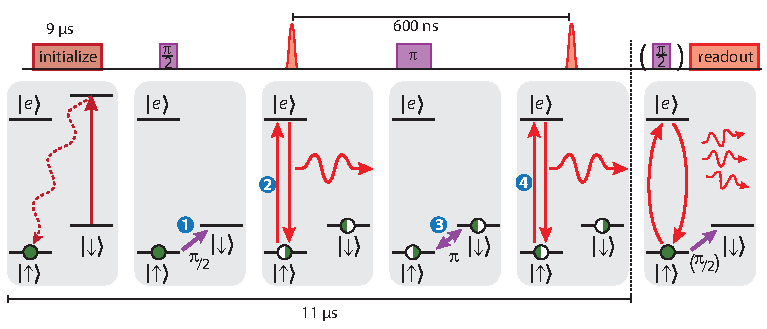
\includegraphics{fig1_entanglement_protocol}
	\caption{\label{fig:LDE-fig1-protocol} \textbf{Protocol.} Entanglement protocol (details in main text), illustrating the pulse sequence applied simultaneously to both NV centres. Both NV centres are initially prepared in a superposition $1/\sqrt{2}(\ket{\up}+\ket{\down})$. A short $2\,$ns spin-selective resonant laser pulse creates spin-photon entanglement $1/\sqrt{2}(\ket{\uparrow 1}+\ket{\downarrow 0})$. The photons are overlapped on the beamsplitter and detected in the two output ports. Both spins are then flipped, and the NV centres are excited a second time. The detection of one photon in each excitation round heralds the entanglement and triggers individual spin readout.}
\end{figure}

Any realistic experiment, however, suffers from photon loss and imperfect detector efficiency; detection of a single photon is thus also consistent with creation of the state $\uu$. To eliminate this possibility, both qubits are flipped and optically excited for a second time. Since $\uu$ is flipped to $\dd$, no photons are emitted in the second round for this state. In contrast, the states $\ket{\psi}$ will again yield a single photon. Detection of a photon in both rounds thus heralds the generation of an entangled state. The second round not only renders the protocol robust against photon loss, but it also changes $\varphi$ into a global phase, making the protocol insensitive to the optical path length difference~\cite{Barrett_Phys.Rev.A_2005} (see Supporting Material). Furthermore, flipping the qubits provides a refocusing mechanism that counteracts spin dephasing during entanglement generation. The final state is one of two Bell states $\ket{\psi^\pm}=1/\sqrt{2}(\ket{\uparrow_\text{A}\downarrow_\text{B}}\pm\ket{\downarrow_\text{A}\uparrow_\text{B}})$, with the sign depending on whether the same detector ($+$), or different detectors ($-$) clicked in the two rounds.

\subsection{Implementation}

A key challenge for generating remote entanglement with solid-state qubits is obtaining a large flux of indistinguishable photons, in part because local strain in the host lattice can induce large variations in photon frequency. The optical excitation spectra of the NV centres (Fig.~\ref{fig:LDE-fig2}a) display sharp spin-selective transitions. Here we use the $E_\text{y}$ transition (spin projection $\mszero$) in the entangling protocol and for qubit readout; we use the $A_1$ transition for fast optical pumping into $\ket{\up}$~\cite{Robledo_Nature_2011}. Due to different strain in the two diamonds, the frequencies of the $E_\text{y}$ transitions differ by 3.5$\,$GHz, more than 100 line-widths. By applying a voltage to an on-chip electrode (Fig.~\ref{fig:LDE-fig1-setup}b) we tune the optical transition frequencies of one centre (NV~B) through the d.c. Stark effect~\cite{Bernien_Phys.Rev.Lett._2012,Bassett_Phys.Rev.Lett._2011} and bring the $E_\text{y}$ transitions of the two NV centres into resonance (Fig.~\ref{fig:LDE-fig2}a bottom).

\begin{figure}[tp]
	\centering
	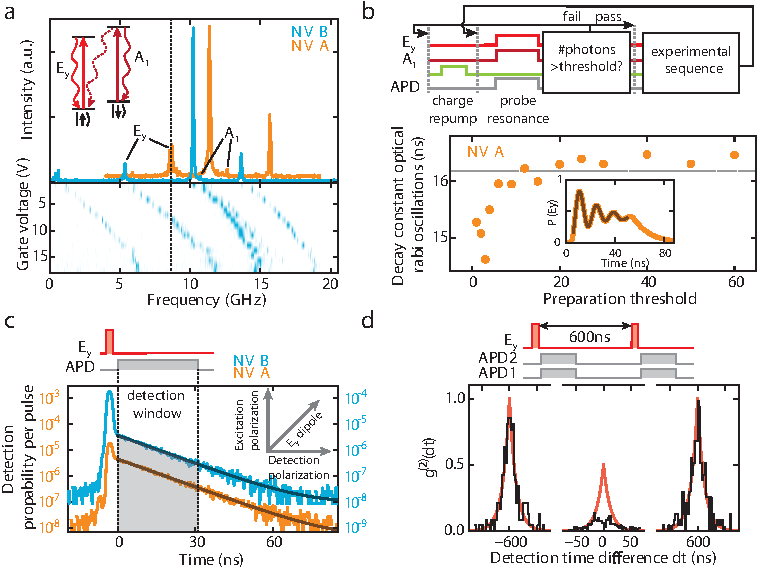
\includegraphics{fig2_ind_photons}
	\caption{\label{fig:LDE-fig2} \textbf{Generating and detecting indistinguishable photons.}
	\textbf{a,} Excitation spectra; frequency relative to 470.4515$\,$THz. By applying a voltage to the gates of NV~B the $E_\text{y}$ transitions are tuned into resonance. 
	\textbf{b,} Dynamical preparation of charge and optical resonance. Top: Preparation protocol. A 10$\,\mu$s green laser pulse pumps the NV into its negative charge state~\cite{Robledo_Nature_2011}. The transition frequencies are probed by exciting the $E_\text{y}$ and $A_\text{1}$ transitions for 60$\,\mu$s. Conditional on surpassing a certain number of photons detected the experiment is started (pass) or preparation is repeated (fail). APD, avalanche photodiode. Bottom: Line-narrowing effect of the preparation shown by the dependence of the decay time of optical Rabi oscillations on preparation threshold. Dashed line indicates lifetime-limited damping~\cite{Robledo_Phys.Rev.Lett._2010}. 
	% For the entanglement experiment we choose a threshold of 45 (20) photons for NV~A (NV~B). 
	\textbf{c,} Resonant optical excitation and detection. The polarisation axis of the detection path is aligned perpendicular to the excitation axis. The dipole axis of the $E_\text{y}$ transition is oriented in between these two axes (inset). Remaining laser light reflection is time-filtered by defining a photon detection window that starts after the laser pulse. 
	\textbf{d,} Two-photon quantum interference using resonant excitation and detection. The $g^{(2)}$ correlation function is obtained from all coincidence detection events of APD~1 and APD~2 during the entanglement experiment (see Supporting Material). The side-peaks are fit to an exponential decay; from the fit values, we obtain the expected central peak shape $g_\perp^{(2)}$ (red line) for non-interfering photons. The visibility of the interference is given by $(g_\perp^{(2)}-g^{(2)})/g_\perp^{(2)}$.}
\end{figure}


Charge fluctuations near the NV centre also affect the optical frequencies. To counteract photo-ionisation we need to regularly apply a green laser pulse to re-pump the NV centre into the desired charge state. This re-pump pulse changes the local electrostatic environment, leading to jumps of several line-widths in the optical transition frequencies~\cite{Robledo_Phys.Rev.Lett._2010}. To overcome these effects, we only initiate an experiment if the number of photons collected during a two-laser probe stage (Fig.~\ref{fig:LDE-fig2}b) exceeds a threshold, thereby ensuring that the NV centre optical transitions are on resonance with the lasers (see chapter~\ref{sec:CR-verification}). The preparation procedure markedly improves the observed optical coherence: as the probe threshold is increased, optical Rabi oscillations persist for longer times (see Fig.~\ref{fig:LDE-fig2}b). For high thresholds, the optical damping time saturates around the value expected for a lifetime-limited line-width~\cite{Robledo_Phys.Rev.Lett._2010}, indicating that the effect of spectral jumps induced by the re-pump laser is strongly mitigated.

Besides photon indistinguishability, successful execution of the protocol also requires that the detection probability of resonantly emitted photons exceeds that of scattered laser photons and of detector dark counts. This is particularly demanding for NV centres since only about 3\% of their emission is in the zero-phonon line and useful for the protocol. To minimise detection of laser photons, we use both a cross-polarised excitation-detection scheme (Fig.~\ref{fig:LDE-fig2}c inset) and a detection time filter that exploits the difference between the length of the laser pulse (2$\,$ns) and the NV centre's excited state lifetime (12\,ns) (Fig.\,\ref{fig:LDE-fig2}c). For a typical detection window used, this reduces the contribution of scattered laser photons to about 1\%. Combined with micro-fabricated solid-immersion lenses for enhanced collection efficiency (Fig.~\ref{fig:LDE-fig1-setup}b) and spectral filtering for suppressing non-resonant NV emission, we obtain a detection probability of a resonant NV photon of about $4\times10^{-4}$ per pulse --- about 70 times higher than the sum of background contributions.

The degree of photon indistinguishability and background suppression can be obtained directly from the second-order autocorrelation function $g^{(2)}$, which we extract from our entanglement experiment (see Supporting Material). For fully distinguishable photons, the value of $g^{(2)}$ would reach 0.5 at zero arrival time difference. A strong deviation from this behaviour is observed (Fig.~\ref{fig:LDE-fig2}d) due to two-photon quantum interference~\cite{Hong_Phys.Rev.Lett._1987} that, for perfectly indistinguishable photons, would make the central peak fully vanish. The remaining coincidences are likely caused by (temperature-dependent) phonon-induced transitions between optically excited states~\cite{Fu_Phys.Rev.Lett._2009} in NV~A. The visibility of the two-photon interference observed here --- $(80\pm5)$\% for $|dt| < 2.56\,$ns --- is a significant improvement over previously measured values~\cite{Bernien_Phys.Rev.Lett._2012,Sipahigil_Phys.Rev.Lett._2012} and key to the success of the entangling scheme.

To experimentally generate and detect remote entanglement, we run the following sequence: First, both NV centres are independently prepared into the correct charge state and brought into optical resonance according to the scheme in figure~\ref{fig:LDE-fig2}b. Then we apply the entangling protocol shown in figure~\ref{fig:LDE-fig1-protocol} using a 600$\,$ns delay between the two optical excitation rounds. We repeat the protocol 300 times before we return to the resonance preparation step; this number is a compromise between maximising the attempt rate and minimising the probability of NV centre ionisation. A fast logic circuit monitors the photon counts in real time and triggers single-shot qubit readout on each setup whenever entanglement is heralded, i.e. whenever a single photon is detected in each round of the protocol. The readout projects each qubit onto the \{$\ket{\up}$, $\ket{\down}$\} states (Z-basis), or on the \{$\ket{\up} \pm \ket{\down}$, $\ket{\up} \mp \ket{\down}$\} states (X or $-$X basis). The latter two are achieved by first rotating the qubit by $\pi/2$ using a microwave pulse before readout. By correlating the resulting single-qubit readout outcomes we can verify the generation of the desired entangled states. To obtain reliable estimates of the two-qubit state probabilities, we correct the raw data with a maximum-likelihood method for local readout infidelities. These readout errors are known accurately from regular calibrations performed during the experiment (see Supporting Material).

\subsection{Demonstration of remote entanglement}

Figure~\ref{fig:LDE-fig3} shows the obtained correlations. When both qubits are measured along Z (readout basis \{Z,Z\}), the states $\psi^+$ and $\psi^-$ (as identified by their different photon signatures) display strongly anti-correlated readout results (odd parity). The coherence of the joint qubit state is revealed by measurements performed in rotated bases (\{X,X\}, \{$-$X,X\}), which also exhibit significant correlations. Furthermore, these measurements allow us to distinguish between states $\psi^+$ and $\psi^-$. For $\psi^+$ the \{X,X\} (\{$-$X,X\}), outcomes exhibit even (odd) parity, whereas the $\psi^-$ state displays the opposite behaviour, as expected. The observed parities demonstrate that the experiment yields the two desired entangled states.

\begin{figure}[tp]
	\centering
	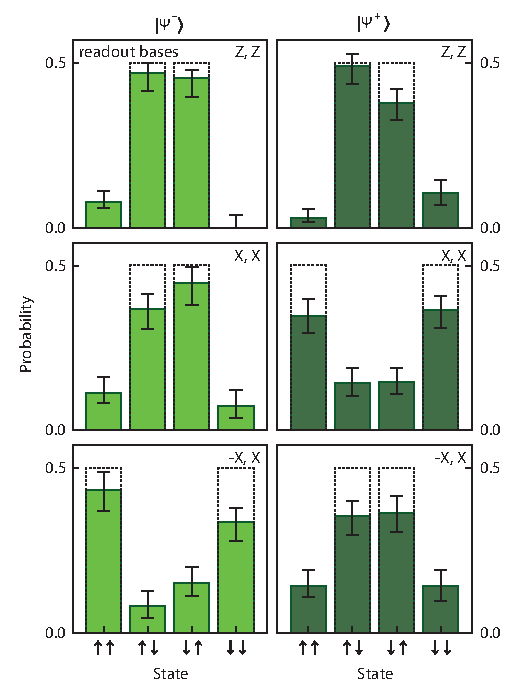
\includegraphics{H_Bernien_fig3}
	\caption{\label{fig:LDE-fig3} \textbf{Verification of entanglement by spin-spin correlations.} Each time that entanglement is heralded the spin qubits are individually read out and their results correlated. The readout bases for NV~A and NV~B can be rotated by individual microwave control (see text). The state probabilities are obtained by a maximum-likelihood estimation on the raw readout results (see Supporting Material). Error bars depict 68\% confidence intervals; dashed lines indicate expected results for perfect state fidelity. Data is obtained from 739 heralding events. For $\psi^-$, the detection window in each round is set to 38.4$\,$ns, and the maximum absolute detection time difference $|\delta\tau|$ between the two photons relative to their laser pulses is restricted to 25.6$\,$ns. $\delta\tau=\tau_2-\tau_1$, where $\tau_1$ is the arrival time of the first photon relative to the first laser pulse and $\tau_2$ the arrival time of the second photon relative to the second laser pulse. For $\psi^+$ the second detection window is set to 19.2$\,$ns with $|\delta\tau|<12.8\,$ns, in order to reduce the effect of photo-detector after-pulsing.}
\end{figure}

We calculate a strict lower bound on the state fidelity by combining the measurement results from different bases (see Supporting Material):
\begin{equation}\label{eq:LDE_LB}
F = \langle\psi^\pm|\rho|\psi^\pm \rangle \geq \ 1/2(P_{\uparrow\downarrow}+P_{\downarrow\uparrow}+C)-\sqrt{P_{\uparrow\uparrow}P_{\downarrow\downarrow}},
\end{equation}
where $P_{ij}$ is the probability for the measurement outcome $ij$ in the \{Z,Z\} basis (i.e. the diagonal elements of the density matrix $\rho$) and $C$ is the contrast between odd and even outcomes in the rotated bases. We find a lower bound of $(69\pm5)$\% for $\psi^-$ and $(58\pm6)$\% for $\psi^+$, and probabilities of 99.98\% and 91.8\%, respectively, that the state fidelity is above the classical limit of 0.5. These values firmly establish that we have created remote entanglement.

The lower bound on the state fidelity given above takes into account the possible presence of coherence within the even-parity subspace \{$\uu$, $\dd$\}. However, the protocol selects out states with odd parity and therefore this coherence is expected to be absent. To compare the results to the expected value and to account for sources of error, we set the related (square-root) term in Eq. 1 to zero and obtain for the data in figure~\ref{fig:LDE-fig3} as best estimate $F=(73\pm4)$\% for $\psi^-$ and $F=(64\pm5)\%$ for $\psi^+$.

Several known error sources contribute to the observed fidelity. Most importantly, imperfect photon indistinguishability reduces the coherence of the state. The fidelity is further decreased by errors in the microwave pulses (estimated at 3.5\%), spin initialisation (2\%), spin decoherence ($<1$\%) and spin flips during the optical excitation (1\%) (see Supporting Material). Moreover, $\psi^+$ is affected by after-pulsing, whereby detection of a photon in the first round triggers a fake detector click in the second round. Such after-pulsing leads to a distortion of the correlations (see for example the increased probability for $\dd$ in figure~\ref{fig:LDE-fig3}) and thereby a reduction in fidelity for $\psi^+$ (see Supporting Material). Besides these errors that reduce the actual state fidelity, the measured value is also slightly lowered by a conservative estimation for readout infidelities and by errors in the final microwave $\pi/2$ pulse used for reading out in a rotated basis.

The success probability of the protocol is given by $P_\psi =1/2 \eta_\text{A}\eta_\text{B}$. $\eta_i$ is the overall detection efficiency of resonant photons from NV $i$ and the factor 1/2 takes into account cases where the two spins are projected into $\dd$ or $\uu$, which are filtered out by their different photon signature. In the current experiment we estimate $P_\psi \approx 1.6 10^{-7}$. The entanglement attempt rate is about 20$\,$kHz, yielding one entanglement event per 10 minutes. This is in good agreement with the 739 entanglement events obtained over a time of 158 hours.

Creation of entanglement between distant spin qubits in diamond, as reported here, opens the door to extending the remarkable properties of NV-based quantum registers towards applications in quantum information science. A natural path forward is the incorporation of auxiliary nuclear spin qubits at the local nodes. In the following we discuss a second experiment where the nitrogen spin initialization and decoherence protected gates (as described in chapter \ref{ch:AMC}) are combined with an improved entanglement protocol to realize a deterministic Bell-state measurement which enables teleportation between a single nuclear spin and a distant electron spin.

\section{Teleportation}

Teleportation allows quantum information to be faithfully transmitted over arbitrary distances provided the two parties (``Alice'' and ``Bob'') have previously established a shared entangled state and can communicate classically.
In the teleportation protocol ( Fig.~\ref{LDE:fig4} ) Alice is initially in possession of the state to be teleported (qubit 1) which is most generally given by $\ket\psi = \alpha\ket0 + \beta\ket1$. Alice and Bob each have one qubit of an entangled pair (qubits 2 and 3) in the joint state $\ket{\Psi^-}_{23} = (\ket{01}_{23} - \ket{10}_{23})/\sqrt2$. The combined state of all three qubits can be rewritten as
\begin{align}
    \ket\psi_1 \otimes \ket{\Psi^-}_{23} = \frac{1}{2} \big( 
        & \ket{\Phi^+}_{12} \otimes (\alpha\ket1_3 - \beta\ket0_3) \nonumber\\
        + & \ket{\Phi^-}_{12} \otimes (\alpha\ket1_3 + \beta\ket0_3) \nonumber\\
        + & \ket{\Psi^+}_{12} \otimes (- \alpha\ket0_3 + \beta\ket1_3) \nonumber\\
        - & \ket{\Psi^-}_{12} \otimes (\alpha\ket0_3 + \beta\ket1_3)
        \big),
\end{align}
where $\ket{\Phi^\pm} = (\ket{00}\pm\ket{11})/\sqrt2$ and $\ket{\Psi^\pm} = (\ket{01}\pm\ket{10})/\sqrt2$ are the four Bell states. To teleport the quantum state Alice performs a joint measurement on her qubits (qubits 1 and 2) in the Bell basis, projecting Bob's qubit into a state that is equal to $\ket\psi$ up to a unitary operation that depends on the outcome of Alice's measurement. Alice sends the outcome via a classical communication channel to Bob, who can then recover the original state by applying the corresponding local transformation.

Because the source qubit state always disappears on Alice's side, it is irrevocably lost whenever the protocol fails. Therefore, to ensure that each qubit state inserted into the teleporter unconditionally re-appears on Bob's side, Alice must be able to distinguish between all four Bell states in a single shot and Bob has to preserve the coherence of the target qubit during the communication of the outcome and the final conditional transformation. Several pioneering experiments have explored teleportation between remote nodes~\cite{Olmschenk_Science_2009,Nolleke_Phys.Rev.Lett._2013,Krauter_NatPhys_2013} but unconditional teleportation between long-lived qubits~\cite{Awschalom_Science_2013,Devoret_Science_2013,Monroe_Science_2013} has so far only been demonstrated within a local qubit register~\cite{Riebe_Nature_2004,Barrett_Nature_2004,Steffen_Nature_2013}.

\begin{figure*}
    \centering
    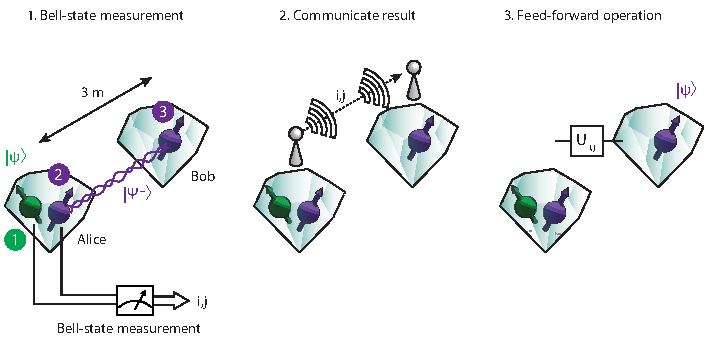
\includegraphics{fig4_teleportation_scheme}
    \caption{
    \label{LDE:fig4} 
    \textbf{Teleportation scheme.} 
    General scheme for teleportation. In our experiment Alice and Bob each control a single NV center in a single-crystal CVD-grown diamond by operating an independent cryogenic confocal microscope setup (T = 8\,K for Alice and T  = 4\,K for Bob). 
    % See supplementary methods for details.
    }
\end{figure*}

We demonstrate unconditional teleportation between diamond spin qubits residing in independent setups separated by 3 meters. This result is achieved by fully separating the generation of remote entanglement (the preparation of the teleporter) as from the two-qubit Bell-state measurement and feed-forward (the actual teleportation action). In particular, a photonic channel is used to generate heralded remote entanglement between two nitrogen-vacancy (NV) center electronic spins, while the teleportation protocol solely exploits matter qubits that – unlike photonic qubits – allow for a deterministic Bell-state measurement with current technology. The source state is encoded in a nuclear spin close to one of the NV electron spins after preparation of the teleporter. We preserve the target qubit's coherence by dynamical decoupling while the measurement outcome is forwarded and the final correction pulse is applied. This protocol ensures that the source state is successfully teleported in each of the experimental runs.

Alice and Bob each operate an independent low-temperature confocal microscope setup that addresses a single NV center. The two NV electronic spins (labeled as qubits 2 and 3) are initialized in the non-local entangled state $\ket{\Psi^-}_{23} = (\ket{01}_{23} - \ket{10}_{23})/\sqrt2$ according to the protocol described in~\ref{sec:HE}, with the following improvements: We have further enhanced the efficiency of photon collection from our device through optimization of the SIL fabrication and by adding an anti-reflection coating. Also, we have significantly improved both the spectral stability of the NV center's optical transition and the charge state initialization by resonant re-pumping on the neutral-charge state zero-phonon line~\cite{Siyushev_Phys.Rev.Lett._2013}. As a result we were able to increase the generation rate of the entangled state $\ket{\Psi^-}_{23}$ fivefold to $1/250\, \mathrm s^{-1}$ and improve the entangled state fidelity from 0.73 to an estimated 0.87.

\begin{figure*}
	\centering
    \includegraphics{fig5_Prepare_teleporter}
    \caption{
    \label{fig:LDE-fig5} 
    \textbf{Preparation of the teleporter.}
    (a) Circuit diagram for the periodic measurement-based re-initialization of the nuclear spin (qubit 1) in between remote entanglement generation attempts. Both the probability for success per attempt and the time duration of a single attempt are indicated for the initialization by measurement of qubit 1 and the generation of entanglement between qubits 2 and 3. 
    (b) Measured probability P($\ket1$) to preserve the initialized nuclear spin state $\ket1$ as a function of number of entanglement generation attempts $N_\text{ent}$. A fit (solid line) to a rate-equation model yields a probability of $(0.85 \pm 0.05) \times 10^{-3}$ per entanglement generation attempt that the nuclear spin flips. The dashed line marks the maximum number of attempts before the nuclear spin is re-initialized ($N_\text{ent} = 250$). }
\end{figure*}



The additional qubit in Alice's node --- essential for making the teleportation unconditional --- is provided by the nitrogen-14 nuclear spin of Alice's NV (qubit 1). Before establishing the entanglement link, this nuclear spin is initialized into state $\ket1$ by a projective measurement via the electron spin~\cite{Robledo_Nature_2011}. We reinitialize the nuclear spin after each 250 entanglement attempts in order to preserve its purity (Figs.~\ref{fig:LDE-fig5}a,b). We prepare the source state after establishing remote entanglement, thus avoiding possible dephasing of the source state by repeated optical excitation of the nearby electron~\cite{Jiang_Phys.Rev.Lett._2008,Blok_NatPhys_2014} during entanglement generation. We employ a decoherence-protected gate~\cite{vanderSar_Nature_2012} on Alice's side to set the nuclear spin to the source state $\ket\psi = \alpha\ket0 + \beta\ket1$. This gate combines two nuclear spin rotations with a refocusing pulse on the electron spin such that the entangled state is efficiently preserved for the duration of the gate (Figs.~\ref{fig:LDE-fig6}a). This operation concludes the preparation of the teleporter and the insertion of the source qubit, with the three-qubit system left in the state $\ket\psi_1 \otimes \ket{\Psi^-}_{23} = (\alpha\ket0_1 + \beta\ket1_1) \otimes (\ket{01}_{23} - \ket{10}_{23})/\sqrt2$.

\begin{figure*}
	\centering
    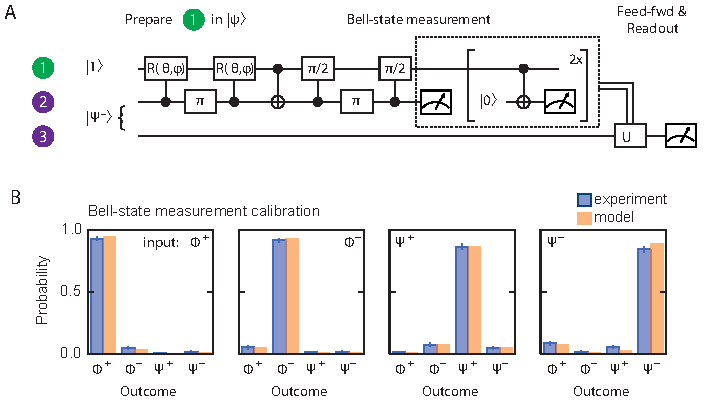
\includegraphics{fig6_circuit_diagram_bell_state_measurement}
    \caption{
    \label{fig:LDE-fig6} 
    \textbf{Deterministic Bell-state measurement (BSM) and real-time feed-forward.}
    (a) Circuit diagram of our implementation. The label `e' (`N') indicates operations acting on the electron spin (nitrogen nuclear spin). To enhance the readout fidelity for the nuclear spin, we perform the mapping to the electron spin via a CNOT and the subsequent electron readout twice. While Alice is performing her BSM Bob applies an XY4 decoupling sequence on his electron qubit. After receiving the BSM outcome from Alice, Bob applies the feed-forward operation $U$ and reads out his qubit. $\pi_{x,y}$ denote rotations around the $x$-axis and $y$-axis, respectively. 
    (b) Calibration of the BSM by inserting the four different Bell states on Alice's side and determining the probability with which the ideal outcome is observed (blue bars). Data is not corrected for imperfect preparation of the input states. Expectations based on independently determined experimental imperfections are shown in orange. Error bars are two statistical s.d.
    }
\end{figure*}


At the heart of unconditional qubit teleportation is a deterministic Bell-state measurement (BSM) by Alice on qubits 1 and 2 that generally involves two steps. First, the four Bell states are mapped onto the four different qubit eigenstates $\ket{i}_1 \ket{j}_2$ by quantum gate operations. In the second step each of the two qubits is read out in a single shot and the two measurement outcomes are sent to Bob. Our implementation of this scheme is shown in Figs.~\ref{fig:LDE-fig6}a. We implement the Bell-state mapping by applying a two-qubit controlled-NOT gate (CNOT) followed by a $\pi/2$ rotation on the nuclear spin using another decoherence-protected gate. Then we read out the electron spin in a single shot (average fidelity $0.963\pm0.005$). Finally we read out the nuclear spin by mapping its state onto the electron spin followed by electron spin readout. The two single-shot readout results give the outcome of the BSM.

We benchmark the BSM by preparing each of the four Bell states as input states in Alice's register (Fig.~\ref{fig:LDE-fig6}b). This procedure yields an uncorrected mean fidelity, given by the probability to obtain the measurement result corresponding to the prepared Bell state, of $0.89\pm0.02$. To gain more insight into the sources of imperfections we compare the data with numerical simulations that use the independently determined infidelities of the nuclear spin initialization, CNOT gate, and electron single-shot readout as input. These simulations predict an average fidelity of 0.9 (Fig.~\ref{fig:LDE-fig6}b), in excellent agreement with the data. Taking known errors in the preparation of the input states into account, we infer a BSM fidelity of $0.93\pm0.02$.

The final challenge for successful unconditional teleportation is to maintain the coherence of Bob's target qubit (qubit 3) during the BSM and feed-forward. In our experiment, Bob's qubit is mostly affected by interactions with the surrounding nuclear spin bath. We counteract this decoherence by applying an XY4 dynamical decoupling sequence~\cite{Lange_Science_2010}. The time between entanglement generation and the triggering of the feed-forward operation based on the BSM outcome is 300\,\textmicro s. For this duration the decoupling protocol preserves the qubit state with an average fidelity of $0.96\pm0.02$.

We first verify that the teleporter is calibrated correctly by applying it to the nominal input state $\ket Y = (\ket0+\ii\ket1)/\sqrt2$ and performing tomography on the state that appears on Bob's side. The reconstructed density matrix (Fig.~\ref{fig:LDE-fig7}B) shows that the target state vector is aligned well with $Y$ and therefore that the reference frames of Alice and Bob are correctly set.

\begin{figure*}
	\centering
    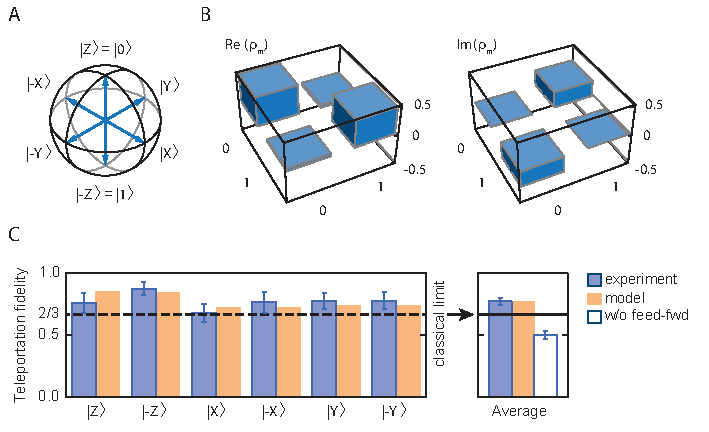
\includegraphics{fig7_teleportation_data}
    \caption {
    \label{fig:LDE-fig7} 
    \textbf{Demonstration of unconditional quantum teleportation between remote qubits.}
    (a) Bloch sphere with the six mutually unbiased basis states that we teleport. $\ket{\pm X} = (\ket0 \pm \ket1)/\sqrt2$, $\ket{\pm Y} = (\ket0 \pm \ii \ket1)/\sqrt2$.
    (b) State tomography after teleportation of the input state $\ket Y$. We determine the density matrix $\rho_\mathrm m$ by measuring the expectation values of the Pauli spin operators, $\langle \sigma_x \rangle$, $\langle \sigma_y \rangle$, $\langle \sigma_z \rangle$, where the required qubit rotations before readout are performed conditional on the BSM outcome. The measured (ideal) entries of the density matrix are $\rho_{00} = 1 - \rho_{11} = 0.52 \pm 0.08 \; (0.5)$ and $\rho_{01} = \rho_{10}^* = 0.05 \pm 0.08 - \ii 0.28 \pm \ii 0.07\; (- \ii 0.5)$, respectively.
    (c) Average teleportation fidelity from the measured fidelities of the six states (blue bars). Sample sizes are (left to right) 54, 89, 73, 49, 52, and 47. Predictions from simulations are shown in orange. Without feed-forward, the target state is completely mixed (white bar). The horizontal line marks the classical limit of $2/3$. Data is not corrected for source state initialization errors. Uncertainties are one statistical s.d. 
    }
\end{figure*}
To prove that our quantum teleporter outperforms any classical communication strategy, we teleport an unbiased set of six basis states $\ket\psi$ (Fig.~\ref{fig:LDE-fig7}A) and determine the fidelity of the teleported state on Bob's side with respect to the ideal input state. In these experiments we use a feed-forward operation that maps the ideal state of qubit 3 onto a qubit eigenstate such that the readout directly yields the teleportation fidelity. Since the feed-forward operation is conditional on the BSM outcome, ignoring the BSM outcome yields a completely mixed state and random outcomes ensuring that no information is transmitted. Without feed-forward we indeed observe an average teleportation fidelity of $\langle F \rangle = 0.50 \pm 0.03$ (Fig.~\ref{fig:LDE-fig7}C). In contrast, including the feed-forward loop we find $\langle F \rangle = 0.77 \pm 0.03$. This value exceeds the classical limit of $2/3$ by more than 3 standard deviations, thus proving the quantum nature of our teleporter. We note that this fidelity presents a lower bound on the actual teleportation fidelity because it does not take into account initialization errors of the source state. Importantly, this result is obtained without any post-selection: each teleportation attempt is included in the data presented here.

We also simulate the outcomes by using independently determined infidelities in the protocol. The only unknown parameter is the fidelity of the entangled state shared by Alice and Bob. We find that our data is well reproduced by the simulations if we assume a fidelity to the ideal Bell state $\ket{\Psi^-}_{23}$ of 0.87 (Fig.~\ref{fig:LDE-fig7}C). The simulations also enable us to quantify the effect of imperfect initialization of the source qubit on the measured fidelities. In this way we estimate the teleportation fidelity to be $\sim 0.86$.

The ability to generate remote entanglement and to control and read out multiple qubits per node as shown in the present teleportation experiment makes NV centers a leading candidate for realizing a quantum network. Our teleportation scheme is both unconditional and scalable to large distances as it can mitigate photon loss by heralding and purification of the distributed entangled state~\cite{Briegel_Phys.Rev.Lett._1998}. In future experiments we aim to supplement our current capabilities with quantum memories that are robust against optical excitation of the electrons, enabling remote entanglement purification and the connection of multiple nodes into the network. A promising route is the use of weakly coupled nuclear spins~\cite{Taminiau_Phys.Rev.Lett._2012,Kolkowitz_Phys.Rev.Lett._2012,Zhao_NatNano_2012} on which multi-qubit quantum control has very recently been demonstrated~\cite{Taminiau_NatNano_2014}. For such nuclear spins, coherence times of over 1 second under optical excitation have been reported~\cite{Maurer_Science_2012}, while the incorporation of NV centers into optical cavities may enable remote entanglement generation on millisecond timescales~\cite{Loncar_MRS_2013}. Furthermore, the entanglement and readout fidelities reported here are sufficient for a violation of a Bell inequality with the detection loophole closed, making NV centers a promising system for realizing a loophole-free Bell test and device-independent quantum key distribution~\cite{Brunner_Rev.Mod.Phys._2014}. 




\clearpage

\bibliographystyle{../thesis}
\bibliography{lde}
